\chapter{Results}
\label{sec:results}

In the current chapter, results of GAT-Denoiser are presented.
First, some small experiments are presented, which do not work on full dataset.
These experiments have been done to find the best suitable architecture and to 
familiarize with the problem and its structure.
Second, a few large experiments are presented, which work on full dataset.
During small and large experiments, some interesting findings are illustrated and GAT-Denoiser
is compared to U-Net and block-matching and 3D filtering (BM3D) \cite{bm3d}.


\section{Dataset}
GAT-Denoiser is tested on lodopab-ct dataset \cite{lodopab-dataset}, which is a 
benchmark dataset for low-dose ct reconstruction methods and therefore well suited for our domain.

The dataset consists of 35820 train images and 3553 test images.
All these images are having resolution 64.

\begin{figure}[H]
  \centering
  \hfill
  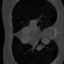
\includegraphics[width=0.2\textwidth]{ct_im_0.png}
  \hfill
  
\includegraphics[width=0.2\textwidth]{ct_im_1.png}
  \hfill
  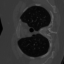
\includegraphics[width=0.2\textwidth]{ct_im_2.png}
  \hfill
  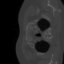
\includegraphics[width=0.2\textwidth]{ct_im_3.png}
  \hfill
  \caption{Some train images of lodopab-ct dataset.}
\end{figure}



\section{Project setup}
Source code of the project is available on GitHub\footnote{https://github.com/cedricmendelin/master-thesis}.

Training of GAT-Denoiser has been done on the HPC-cluster scicore of the University of Basel.
During training, up to 4 titanx GPUs with 12 GB RAM have been used.

\paragraph{Performance metrics}:
During evaluation, two main metrics are used. Further, visual results are presented and can be seen as a third metric.
First, \textit{Loss} is used, which refers to the mean $\ell$-2 distance between original object and reconstruction.
Second, \textit{SNR} is used, which refers to the SNR in dB of reconstruction, compared to original object.

\paragraph{U-Net training:}
As described in section~\ref{sec:unet} \nameref{sec:unet}, a U-Net will be part of our model.
Therefore, U-Net was pre-trained on the lodopab-ct training dataset, with 128 channels in the first contracting step. 
In total, 4 steps have been computed, which results in 1024 channels as output of last contracting step.
During training, noise was sampled from normal distribution to reach SNR in the interval $[0, -10]$ and was added to the observation (sinogram). 
Further, model was trained for 200 iterations.

In the current chapter, we will see how good u-net solely and combined in GAT-Denoiser will perform.

\paragraph{BM3D:}
BM3D is a powerful and lightweight algorithm for image denoising. 
It is not a neural network and was the defacto state-of-the-art before neural network outperformed
BM3D. Therefore, it is an interesting baseline to compare with.

In the GAT-Denoiser pipeline, observations will be denoised and finally, reconstruction takes place.
Therefore, BM3D can be applied at two different steps. First, it can be used to denoise sinogram
and forward denoised sinogram to FBP (basically, that GAT-Denoiser is doing). Secondly, FBP can be
computed with noisy sinogram and the output can be forwarded to BM3D, which will denoised reconstruction.
In the following, term \textit{BM3D sinogram} and \textit{BM3d reconstruction} 
are used to distinguish between the two approaches.


\section{Small Experiments}
For small experiments, not the whole lodopab-ct dataset was used. Only 1024 train images
and 100 validation images have been selected to work with. 
Further, evaluated GAT-Denoiser models have been trained for 200 epochs.

\section{Baseline}

In table~\ref{tab:baseline-small}, baseline results for FBP, BM3D sinogram, BM3D reconstruction and U-Net can be found.
100 images in the test dataset have been used to test the algorithms. Noise was added to the sinograms to reach SNR of 0, -5 and -10 dB.

As expected, reconstruction FBP performs the worst. Then, for lower SNR 0 dB, BM3D outperforms U-Net.
From SNR -5 to -15, U-Net performs best.

\begin{table}[H]
  \centering
  \begin{threeparttable}
    \begin{tabular}{l|cc|cc|cc|cc}
    \toprule
    \textbf{Algorithm} & \multicolumn{2}{l|}{\footnotesize \textbf{Input SNR 0 dB}} & \multicolumn{2}{l|}{\footnotesize \textbf{Input SNR -5 dB}} & \multicolumn{2}{l|}{\footnotesize \textbf{Input SNR -10 dB}} & \multicolumn{2}{l}{\footnotesize \textbf{Input SNR -15 dB}} \\
                       & \textbf{Loss} & \textbf{SNR} & \textbf{Loss} & \textbf{SNR} & \textbf{Loss} & \textbf{SNR} & \textbf{Loss} & \textbf{SNR} \\ 
    \midrule
    FBP                 &  1041.6          &  4.81            & 1772.8         & 0.0           & 3105.6          & -4.96          & 5495.2       & -9.94       \\ \hline
    BM3D sinogram       &  662.2           &  9.30            & 909.5          & 6.13          & 1285.2          & 2.93           & 1884.9       & -0.50       \\ \hline
    BM3D reconstruction &  \textbf{604.2}  &  \textbf{10.15}  & 840.4          & 6.81          & 1283.1          & 2.89           & 2079.1       & -1.42       \\ \hline
    U-Net               &  674.9           &  9.03            & \textbf{711.5} & \textbf{8.17} & \textbf{711.5}  & \textbf{8.17}  & \textbf{1224.9}       & \textbf{3.10}        \\ 
    \midrule
    \end{tabular}

  % \begin{tablenotes}\footnotesize
  %   \item[1] Input SNR 0 dB
  %   \item[2] Input SNR -5 dB
  %   \item[3] Input SNR -10 dB
  %   \item[4] Input SNR -15 dB  
  % \end{tablenotes}
  \end{threeparttable}

  \caption{Baseline results small experiments: Best result in column is marked bold. }
  \label{tab:baseline-small}
\end{table}

  Further, for SNR 0 dB, reconstruction of one test image is illustrated in Figure~\ref{fig:baseline_small}

  \begin{figure}[H]
    \label{fig:baseline_small}
    % \centering
    \hfill
    \subbottom[Clean test image]{
\includegraphics[width=0.15\textwidth]{baseline_small_clean.png}}
    \hfill
    \subbottom[FBP reconstruction]{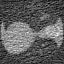
\includegraphics[width=0.15\textwidth]{baseline_small_fbp.png}}
    \hfill
    \subbottom[BM3D sinogram]{
\includegraphics[width=0.15\textwidth]{baseline_small_bm3d_sino.png}}
    \hfill
    \subbottom[BM3D reconstruction]{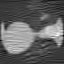
\includegraphics[width=0.15\textwidth]{baseline_small_bm3d_reco.png}}
    \hfill
    \subbottom[U-Net reconstruction]{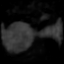
\includegraphics[width=0.15\textwidth]{baseline_small_unet.png}}
    \hfill
	\caption{Example test image baseline reconstructions for input SNR 0 dB}
\end{figure}





  \subsection{Input graph structure}
  In the following Section, experiments with different input graphs are presented.
  As the domain of interest is the input graph, some parameters have been fixed.
  First, U-Net was deactivated, resulting reconstruction is defined as FBP solely.
  Further, GAT-Denoiser has been set to 3 layers, with GAT single head and convolution 
  with one channel, kernel size 3 and padding 1. 
  If nothing else noted, noise was added to reach SNR 0 dB.

  \paragraph{Does learning fail with random graph?}
  Yes it does.

  During experiment, two graphs with size 1024 have been trained.
  First, a k-NN graph with $k=10$, so around 1\%  of all nodes are connected to a single node.
  Second, a random Erdős–Rényi graph with $p=0.01$ has been evaluated, where every node is 
  approximately connected to 1\% of all available nodes.
  
  In the experiment, random Erdős–Rényi graph fails to learn denoising and k-NN starts to capture some details.
  Table~\ref{tab:input_graph} shows Loss and SNR values and in Figure~\ref{fig:input_graph_small} example reconstruction 
  of training example is illustrated.

  \begin{table}[H]
    \centering
      \begin{tabular}{l|cc}
      \toprule
      \textbf{Input graph} & \textbf{Loss} & \textbf{SNR}  \\ 
      \midrule
      Erdős–Rényi graph with $p=0.01$    &  1509.3          &  1.3   \\ \hline
      K-NN graph with $k=10$       &  718.74          &  7.7    \\ \hline
      \midrule
      \end{tabular}
    \caption{Loss and SNR for random graph vs. k-NN graph. }
    \label{tab:input_graph}
  \end{table}
  
  \begin{figure}[H]
    \label{fig:input_graph_small}
    % \centering
    \hfill
    \subbottom[\label{fig:small_experiment_clean2}]{
\includegraphics[width=0.15\textwidth]{baseline_small_clean.png}}
    \hfill
    \subbottom[\label{fig:small_experiment_random_graph}]{
\includegraphics[width=0.15\textwidth]{random__graph_small_experiment.png}}
    \hfill
    \subbottom[\label{fig:small_experiment_knn_graph}]{
\includegraphics[width=0.15\textwidth]{knn__graph_small_experiment.png}}
    \hfill
	\caption{Example test image reconstructions for different input graphs:\\
  Where \ref{fig:small_experiment_clean2} is clean object, 
  \ref{fig:small_experiment_random_graph} reconstruction with  Erdős–Rényi input graph with $p=0.01$ and 
  \ref{fig:small_experiment_knn_graph} reconstruction K-NN input graph with $k=10$.
  }
\end{figure}


  \paragraph{Does result improve with large graph size?}
  Slightly.
  For this questions to answer, multiple models have been trained for graphs with size 512, 1024 and 2048 
  as well as different k-NN parameters (2,6,8,10,20).

  In Table~\ref{tab:graph_knn} results are presented, where Loss, SNR and Training time refer to 
  the average for given graph size. So yes, larger graph size improve our model. 
  But, training is also more expensive regarding training time. 
  Therefore, for all upcoming experiments graph size is fixed to 1024, as it looks like a good
  with good reconstruction result but also not too much training time.
  
  \begin{table}[H]
    \centering
      \begin{tabular}{l|ccc}
      \toprule
      \textbf{Input graph size} & \textbf{Loss} & \textbf{SNR} & \textbf{Training time (s)}  \\ 
      \midrule
      512  &  732.7    &  7.6  & 2678 s \\ \hline
      1024 &  696.1    &  8.1  & 4216 s \\ \hline
      2048 &  628.8    &  8.9  & 7609 s  \\ \hline
      \midrule
      \end{tabular}
    \caption{Loss and SNR for different input graph sizes, which refer to the average of different k-NN parameters.}
    \label{tab:graph_knn}
  \end{table}

  \paragraph{What is a good parameter k for k-NN graph construction?}

  As described in Chapter~\ref{sec:manifold_ct_cryoEM} \textit{\nameref{sec:manifold_ct_cryoEM}},
  it is not easy to determine parameter $k$ in general.
  Therefore, multiple models have been trained with different k (2,6,8,10,20)
  as well as different SNR range (0 dB and -10 dB)


  \textbf{TODO: Recompute values for SNR -10 with training SNR -10 as well }

  In Table~\ref{tab:small_knn_snr}, result of calculated models are illustrated.
  First, input graph resulting from $k=2$ performs surprisingly good for SNR 0 dB.

  \begin{table}[H]
    \centering
    \begin{tabular}{l|cc|cc}
      \toprule
      \textbf{K-NN parameter k} & \multicolumn{2}{l|}{\footnotesize \textbf{Input SNR 0 dB}} & \multicolumn{2}{l|}{\footnotesize \textbf{Input SNR -10 dB}}  \\
                         & \textbf{Loss} & \textbf{SNR} & \textbf{Loss} & \textbf{SNR} \\ 
      \midrule
      2    &  \textbf{609.2}  &  \textbf{9.15}  & 1174.2 & 3.55   \\ \hline
      6    &  650.3           &   8.58          & 1259.3 & 2.87   \\ \hline
      8    &  683.0           &   8.17          & 1135.5 & 3.74   \\ \hline
      10   &  718.7           &   7.72          & 1661.4 & 0.82   \\ \hline
      20   &  819.3           &   6.62          & 1567.2 & 1.19   \\  
      \midrule
    \end{tabular}
  
    \caption{Different k-NN values for validation SNR 0 dB and -10 dB }
    \label{tab:small_knn_snr}
  \end{table}


\subsection{GAT parameters}

\paragraph{How does multiple heads affect result?}
\paragraph{The more layers the better result?}
\paragraph{How about some dropout?}

\subsection{Convolution parameters}
Multiple channels, different kernel-size and padding.

\subsection{Loss}
With 

\subsection{GAT-Denoiser components}



Test many different settings:
\begin{itemize}
  \item K-nn size ([2,4,6,8,10,12]) and sampling points / Graph feature dimension (512, 1024, 1536, 2048)
 
  \item GAT architecute (Layers, Heads, Loss FBP, Fixed conv)
  \item Convolution (with, without, multiple channels)
  \item Loss Sino and FBP
  \item U-Net with and without
  \item Different SNR levels

  
  
\end{itemize}


\section{Large Experiments}
Complete dataset, train for few epochs.

Choose best promising 
